La starup si impone l'obbiettivo di andare a gestire lo scambio di libri all'interno della rete di book-crossing: come visto all'interno dei diversi use-cases, ogni libro nel corso della propria vita all'interno della community, passa di mano in mano attraversando diverse zone.
A questo movimento fisico corrisponde anche un continuo cambio di stato da parte del libro stesso: possiamo riassumere con una \textit{"Finite State Machine"} il percorso che un generico libro segue durante la sua vita.

Riassumendo gli stati di un libro, possono essere:
\begin{itemize}
	\item Out of the network
	\item Available
	\item Under reading
	\item Released
	\item Reserved
	\item Traveling
\end{itemize}

\begin{figure}[h!]
	\centering
	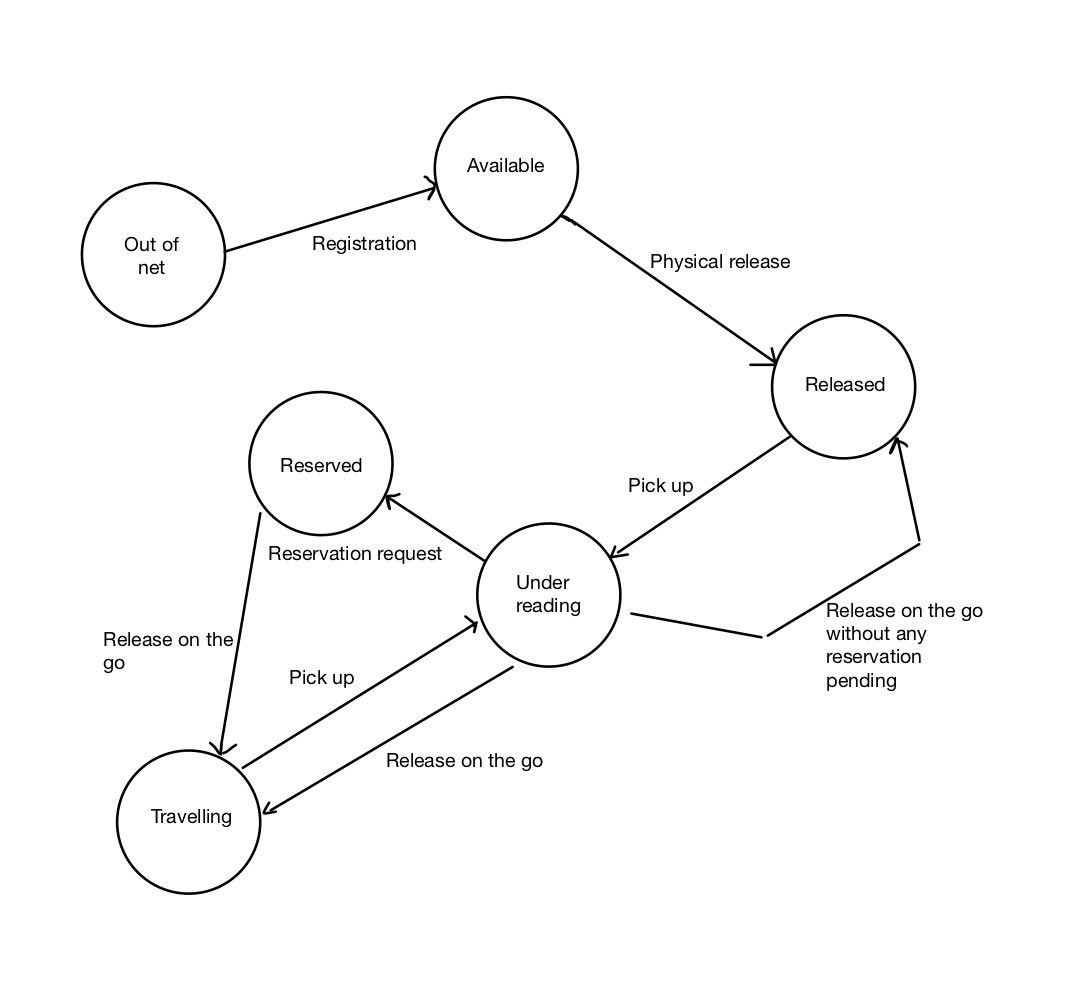
\includegraphics[width=0.6\textwidth]{Immagini/BookState.jpg}
	\caption{Stati del libro all'interno della community}
	\label{fig:BookState}
\end{figure}